\documentclass[11pt,]{article}
\usepackage{lmodern}
\usepackage{amssymb,amsmath}
\usepackage{ifxetex,ifluatex}
\usepackage{fixltx2e} % provides \textsubscript
\ifnum 0\ifxetex 1\fi\ifluatex 1\fi=0 % if pdftex
  \usepackage[T1]{fontenc}
  \usepackage[utf8]{inputenc}
\else % if luatex or xelatex
  \ifxetex
    \usepackage{mathspec}
  \else
    \usepackage{fontspec}
  \fi
  \defaultfontfeatures{Ligatures=TeX,Scale=MatchLowercase}
  \newcommand{\euro}{€}
    \setmainfont[]{IPAPMincho}
    \setsansfont[]{IPAPGothic}
\fi
% use upquote if available, for straight quotes in verbatim environments
\IfFileExists{upquote.sty}{\usepackage{upquote}}{}
% use microtype if available
\IfFileExists{microtype.sty}{%
\usepackage{microtype}
\UseMicrotypeSet[protrusion]{basicmath} % disable protrusion for tt fonts
}{}
\usepackage[margin=1in]{geometry}
\usepackage{hyperref}
\PassOptionsToPackage{usenames,dvipsnames}{color} % color is loaded by hyperref
\hypersetup{unicode=true,
            pdftitle={平成28年度社会医学実習 公衆衛生学担当分},
            pdfauthor={王 超辰},
            colorlinks=true,
            linkcolor=blue,
            citecolor=Blue,
            urlcolor=Blue,
            breaklinks=true}
\urlstyle{same}  % don't use monospace font for urls
\usepackage{graphicx,grffile}
\makeatletter
\def\maxwidth{\ifdim\Gin@nat@width>\linewidth\linewidth\else\Gin@nat@width\fi}
\def\maxheight{\ifdim\Gin@nat@height>\textheight\textheight\else\Gin@nat@height\fi}
\makeatother
% Scale images if necessary, so that they will not overflow the page
% margins by default, and it is still possible to overwrite the defaults
% using explicit options in \includegraphics[width, height, ...]{}
\setkeys{Gin}{width=\maxwidth,height=\maxheight,keepaspectratio}
\setlength{\parindent}{0pt}
\setlength{\parskip}{6pt plus 2pt minus 1pt}
\setlength{\emergencystretch}{3em}  % prevent overfull lines
\providecommand{\tightlist}{%
  \setlength{\itemsep}{0pt}\setlength{\parskip}{0pt}}
\setcounter{secnumdepth}{5}

%%% Use protect on footnotes to avoid problems with footnotes in titles
\let\rmarkdownfootnote\footnote%
\def\footnote{\protect\rmarkdownfootnote}

%%% Change title format to be more compact
\usepackage{titling}

% Create subtitle command for use in maketitle
\newcommand{\subtitle}[1]{
  \posttitle{
    \begin{center}\large#1\end{center}
    }
}

\setlength{\droptitle}{-2em}
  \title{平成28年度社会医学実習 公衆衛生学担当分}
  \pretitle{\vspace{\droptitle}\centering\huge}
  \posttitle{\par}
  \author{王 超辰}
  \preauthor{\centering\large\emph}
  \postauthor{\par}
  \predate{\centering\large\emph}
  \postdate{\par}
  \date{2016年6月23日}


\usepackage{xltxtra}
\XeTeXlinebreaklocale ``ja''
\XeTeXlinebreakskip=0pt plus 1pt
\XeTeXlinebreakpenalty=0

% Redefines (sub)paragraphs to behave more like sections
\ifx\paragraph\undefined\else
\let\oldparagraph\paragraph
\renewcommand{\paragraph}[1]{\oldparagraph{#1}\mbox{}}
\fi
\ifx\subparagraph\undefined\else
\let\oldsubparagraph\subparagraph
\renewcommand{\subparagraph}[1]{\oldsubparagraph{#1}\mbox{}}
\fi

\begin{document}
\maketitle

\section{がんの記述疫学:}

\subsection{目的:}

\begin{enumerate}
\def\labelenumi{\arabic{enumi}.}
\tightlist
\item
  各部位がんのリスク要因を調べる.\\
\item
  年齢,出生コホート,時期効果に関する内容を理解する.
\end{enumerate}

\subsection{方法:}

各部位がんのリスク要因を検索して,できるだけ挙げる.
配布資料を参考した上で,日本のがん登録データをダウロードし,次の各部位のがんを解析する.
各部位がんデータから年齢・出生コホート・時期効果があるかを説明する.

\subsection{課題:}

\begin{enumerate}
\def\labelenumi{\arabic{enumi}.}
\item
  肝がんのリスク要因と死亡データの年齢,出生コホート,時期効果分析
  (Group 1)
\item
  胃がんのリスク要因と死亡データの年齢,出生コホート,時期効果分析
  (Group 2\_菊地先生)
\item
  胆のうがんのリスク要因と死亡データの年齢,出生コホート,時期効果分析
  (Group 3)
\item
  膵がんのリスク要因と死亡データの年齢,出生コホート,時期効果分析
  (Group 4)
\item
  食道がんのリスク要因と死亡データの年齢,出生コホート,時期効果分析
  (Group 5)
\item
  肺がんのリスク要因と死亡データの年齢,出生コホート,時期効果分析
  (Group 6)
\end{enumerate}

\section{参考:}

\begin{enumerate}
\def\labelenumi{\arabic{enumi}.}
\item
  \url{https://rpubs.com/kaz_yos/epi-cross-long}
\item
  テキストの該当部分{[}1{]} Chapter 1: 1.2 (Page 4-14)\\
  pdf download: \url{http://winterwang.github.io/files/textbook.pdf}
\item
  実習用データの入手先:cancer\_mortality(1958-2014).xls {[}2{]}
  \url{http://ganjoho.jp/reg_stat/statistics/dl/index.html}
\end{enumerate}

\section{年齢,出生コホート,時期効果に関する内容の理解}

\begin{itemize}
\tightlist
\item
  年齢効果:\\
  年齢の増加とともに,罹患・死亡率が上昇・減少する.(生まれた年や調査時の年代に関わらず)
\item
  出生コホート効果:\\
  生まれた年により,罹患・死亡率が異なる.(調査時の年代と個人の加齢と関係なく)
\item
  時期効果:\\
  ある時点で,ある集団のすべての世代の罹患・死亡率へ影響を及ぼす大事件.(例:戦争,疫病,即効薬・ワクチン・抗生物質の発売や投与,大規模の移民・難民の移動など)
\end{itemize}

\subsection{Table 1.
ある集団で,1975年から2005年に渡って,10年ごと一度某病気の罹患率を横断的な調査した結果:}\label{table-1.-1975200510}

\begin{itemize}
\tightlist
\item
  変数説明:\\
  group: 年齢世代\\
  midpoint: 世代真ん中の年齢値\\
\item
  それぞれの横断的調査(縦方向)から見ると,年齢の増加につれて,罹患率が下がっているような結果になる.
\end{itemize}


\begin{table}[!htbp] \centering 
  \caption{Same with Page 5 Table 1-2 in the textbook} 
  \label{} 
\begin{tabular}{@{\extracolsep{5pt}} ccccccc} 
\\[-1.8ex]\hline 
\hline \\[-1.8ex] 
 & group & midpoint & s1975 & s1985 & s1995 & s2005 \\ 
\hline \\[-1.8ex] 
1 & 10-19 & $15$ & $17$ & $28$ & $$ & $$ \\ 
2 & 20-29 & $25$ & $14$ & $23$ & $35$ & $$ \\ 
3 & 30-39 & $35$ & $12$ & $19$ & $30$ & $45$ \\ 
4 & 40-49 & $45$ & $10$ & $18$ & $26$ & $40$ \\ 
5 & 50-59 & $55$ & $$ & $15$ & $22$ & $36$ \\ 
6 & 60-69 & $65$ & $$ & $$ & $20$ & $31$ \\ 
7 & 70-79 & $75$ & $$ & $$ & $$ & $27$ \\ 
\hline \\[-1.8ex] 
\end{tabular} 
\end{table}

\subsection{Figure 1: 横断的な年齢効果を可視化した図 (Cross-sectional
effect of age at each survey
year)}\label{figure-1--cross-sectional-effect-of-age-at-each-survey-year}

\begin{itemize}
\tightlist
\item
  実線を見ると,すべての時点の横断調査の結果,罹患率高齢者のほうに減少傾向がある.
\item
  しかし,横断の結果から「加齢するとともに,罹患率が減っている」の結論を出してもいいのか?
\end{itemize}

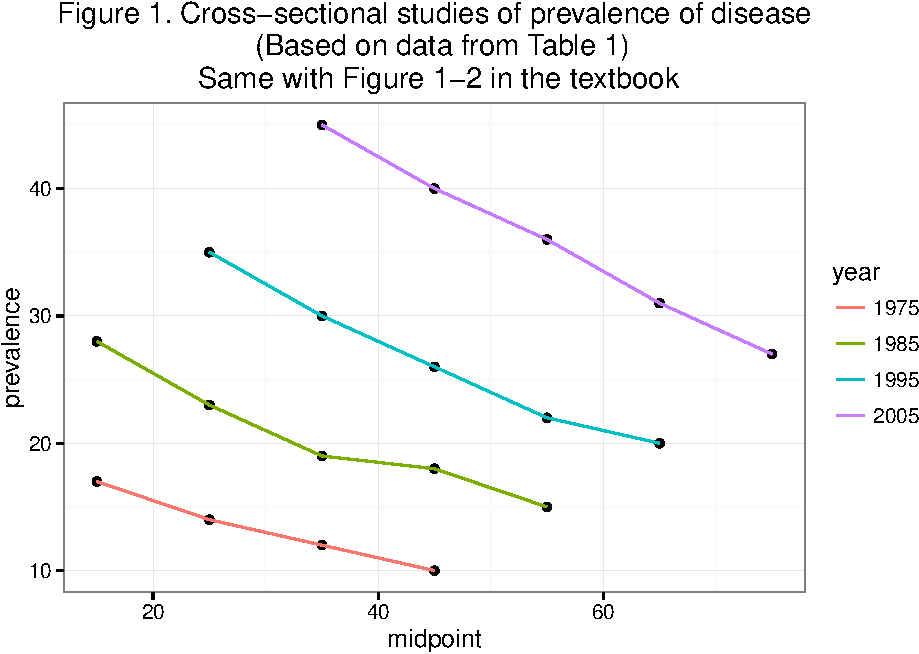
\includegraphics{guidance_files/figure-latex/unnamed-chunk-3-1.pdf}

\subsection{Figure 2
各出生コホートにおいて,縦断的な年齢効果の可視化グラフ (Longitudinal
effect of age for each birth
cohort)}\label{figure-2--longitudinal-effect-of-age-for-each-birth-cohort}

\begin{itemize}
\tightlist
\item
  点線で示したものは,各出生コホートが加齢する(エージング)時の罹患率.
\item
  すべての出生コホートにおいて,加齢とともに,罹患率は増加している.
\end{itemize}

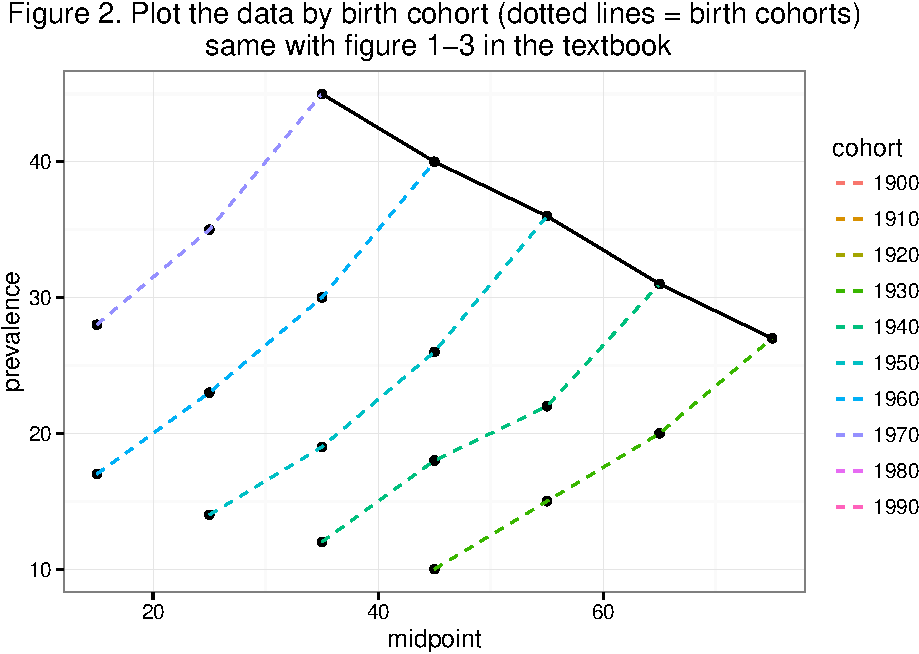
\includegraphics{guidance_files/figure-latex/unnamed-chunk-4-1.pdf}

\subsection{Table 2.
出生コホートによる罹患率を再整理した表}\label{table-2.-}

\begin{itemize}
\tightlist
\item
  出生コホート(横方向)が加齢すると,罹患率は上昇している.
\end{itemize}


\begin{table}[!htbp] \centering 
  \caption{Same with Page 8 Table 1-3 in the textbook} 
  \label{} 
\begin{tabular}{@{\extracolsep{5pt}} cccccccc} 
\\[-1.8ex]\hline 
\hline \\[-1.8ex] 
 & 15 & 25 & 35 & 45 & 55 & 65 & 75 \\ 
\hline \\[-1.8ex] 
1900 & $$ & $$ & $$ & $$ & $$ & $$ & $$ \\ 
1910 & $$ & $$ & $$ & $$ & $$ & $$ & $$ \\ 
1920 & $$ & $$ & $$ & $$ & $$ & $$ & $$ \\ 
1930 & $$ & $$ & $$ & $10$ & $15$ & $20$ & $27$ \\ 
1940 & $$ & $$ & $12$ & $18$ & $22$ & $31$ & $$ \\ 
1950 & $$ & $14$ & $19$ & $26$ & $36$ & $$ & $$ \\ 
1960 & $17$ & $23$ & $30$ & $40$ & $$ & $$ & $$ \\ 
1970 & $28$ & $35$ & $45$ & $$ & $$ & $$ & $$ \\ 
1980 & $$ & $$ & $$ & $$ & $$ & $$ & $$ \\ 
1990 & $$ & $$ & $$ & $$ & $$ & $$ & $$ \\ 
\hline \\[-1.8ex] 
\end{tabular} 
\end{table}

\subsection{Figure 3: 出生コホートごとの罹患率}\label{figure-3-}

\begin{itemize}
\tightlist
\item
  この図は,異常な出生コホートを探すには有利である.
\item
  年齢群を点線で示している.同じ年齢なのに,違う年に生まれたら,罹患率が異なる.(図中には横軸の右方向)
\end{itemize}

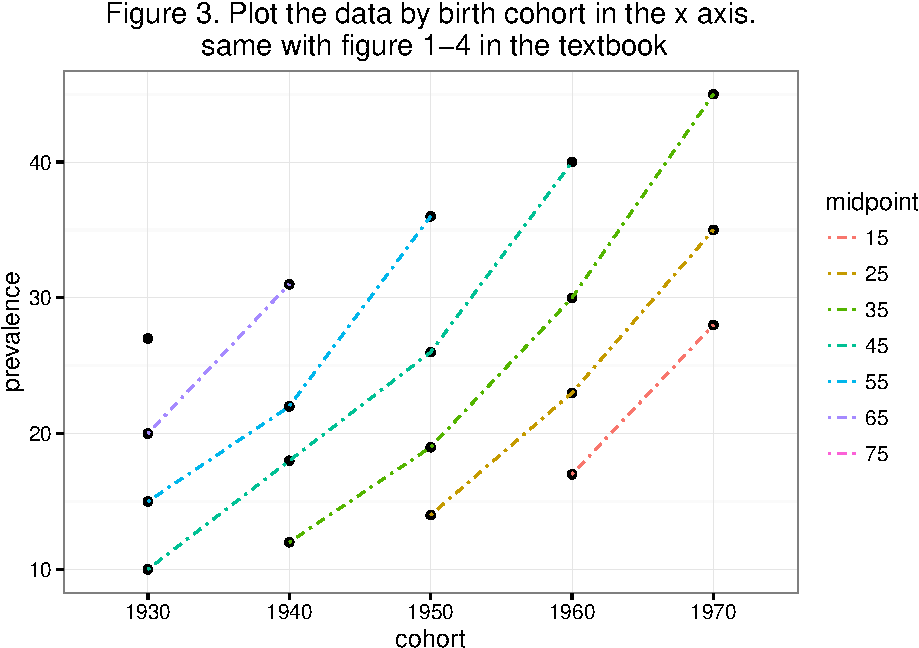
\includegraphics{guidance_files/figure-latex/unnamed-chunk-6-1.pdf}

\section*{参考文献}
\addcontentsline{toc}{section}{参考文献}

\hypertarget{refs}{}
\hypertarget{ref-szkloux5fepidemiology:ux5f2012}{}
{[}1{]} Szklo, M. and Nieto, J. (2012) Epidemiology: Beyond the Basics.
3 edition. Jones \& Bartlett Learning, Burlington, Mass.

\hypertarget{ref-rikan}{}
{[}2{]} 集計表のダウンロード|がん登録・統計[がん情報サービス]
{[}Internet{]}.

\end{document}
